\documentclass[10pt]{article}
\usepackage{homework-style}
\usepackage{pgfplots, tikz}
\pgfplotsset{compat=1.18}


\begin{document}
\dz{7}
\date{20 января 2025}

\begin{tasks}
    \item Докажите, что интервал $(0,1)$ гомеоморфен прямой $\R$. Изометричен ли интервал прямой (метрика на интервале индуцируется из метрики прямой)?
    \begin{proof}
        Возьмём функцию $$f\colon (0;1) \to \R, \quad \theta \mapsto \ctg(\pi(\theta-1)).$$

        Эта функция является непрерывной и биективной. Обратная же функция такова: $$f^{-1}\colon \R \to (0;1), \quad x \mapsto \frac 1 2 - \frac 1 \pi\arctg x.$$

        Она тоже непрерывна.

        \begin{figure}[h]
            \centering
            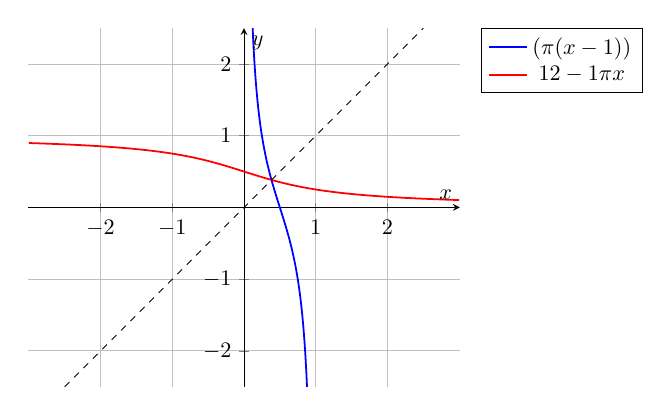
\begin{tikzpicture}[scale=0.8]
                \begin{axis}[
                    axis lines=middle,
                    xlabel={$x$},
                    ylabel={$y$},
                    xmin=-2, xmax=2,  % Set x-axis limits
                    ymin=-2.5, ymax=2.5,  % Set y-axis limits
                    xtick={-2,-1,0,1,2},  % Set x-ticks
                    ytick={-2,-1, 0, 1, 2},  % Set y-ticks
                    grid=both,
                    samples=500,
                    clip=true,  % Prevent clipping
                    axis equal,
                    legend style={at={(1.05,1)}, anchor=north west}  % Position the legend
                ]
                    % Plot the cot(pi(x-1)) function with a label
                    \addplot[blue, thick, domain=0.01:0.99] {cot(deg(pi*(x-1)))}; 
                    \addlegendentry{$\ctg(\pi(x-1))$}  % Label for the cotangent function
                    
                    % Plot the inverse cotangent function with a label
                    \addplot[red, thick, domain=-3:3] {0.5 - (1/pi) * rad(atan(x))};
                    \addlegendentry{$\rfrac 1 2 - \rfrac 1 \pi\arctg x$}  % Label for the inverse cotangent function
    
                    % Plot y=x line with a label
                    \addplot[dashed, domain=-2.5:2.5] {x};
                \end{axis}
            \end{tikzpicture}
        \end{figure}

        Про изометрию можно и не мечтать, ведь если на прямой введена обычная метрика. Тогда на прямой есть точки на расстоянии 100, а на $(0;1)$ нет.
    \end{proof}
    \pagebreak
    \item Докажите, что метрики $\rho_1$, $\rho_2$ и $\rho_\infty$ (см. задачу 2 из ДЗ 6) эквивалентны в том смысле, что $\R^2$ с этими тремя метриками гомеоморфны.
    \begin{proof}[Решение]
        \phantom{sfafd}
        
        \begin{minipage}[b]{0.9\linewidth}
            \begin{lemma}
                Метрические пространства $(X, \rho_1)$ и $(X, \rho_2)$ эквивалентны, если \[\forall x,y \in X\quad\exists L_1, L_2 \in \R\colon \quad L_1 \rho_1(x,y) \leqslant \rho_2(x,y) \leqslant L_2\rho_1(x, y).\]
            \end{lemma}
            \begin{proof}
                Действительно, тогда отображения $\id_X$ и $\id_X^{-1}$ окажутся $L_1$- и $L_2$-липшицевыми соответственно и $\id_X$ --биекция.
            \end{proof}
        \end{minipage}
        
        \begin{conditions}
            \item Докажем, что $\rho_1 \sim \rho_\infty$. Пусть $x=(x_1,x_2),\; y=(y_1, y_2) \in \R^2$, тогда \[\underbrace{\max_{i\in\{1, 2\}}|x_i-y_i|}_{\rho_\infty(x,y)}\leqslant\underbrace{\vphantom{\max_{t\in\{x, y\}}}|x_1-x_2| + |y_1-y_2|}_{\rho_1(x,y)}\leqslant\underbrace{2\cdot\max_{i\in\{1, 2\}}|x_i-y_i|.}_{2\cdot\rho_\infty(x,y)}\]
            \item Докажем, что $\rho_2 \sim \rho_{\infty}$. Также пусть $x =(x_1,x_2),\;y=(y_1, y_2) \in \R^2$, тогда \[
                \underbrace{\vphantom{\sqrt{2\cdot\left(\max_{i\in\{1, 2\}}|x_i-y_i|\right)^2}}\max_{i\in\{1, 2\}}|x_i-y_i|}_{\rho_\infty(x,y)}\leqslant\underbrace{\vphantom{\sqrt{2\cdot\left(\max_{i\in\{1, 2\}}|x_i-y_i|\right)^2}}\sqrt{(x_1-y_1)^2+(x_2-y_2)^2}}_{\rho_2(x,y)}\leqslant \underbrace{\sqrt{2\cdot\left(\max_{i\in\{1, 2\}}|x_i-y_i|\right)^2}}_{\sqrt2 \cdot \rho_\infty(x,y).}
            \]
            \item $\rho_1 \sim \rho_{\infty}$ и $\rho_2 \sim \rho_\infty$, значит $\rho_2 \sim \rho_1$, т.к. отношение $\sim$ является отношением эквивалентности. 
        \end{conditions}
    \end{proof}
    \item Рассмотрим семейство $(A_\lambda)_{\lambda\in\Lambda}$ связных подпространств некоторого топологического пространства. Докажите, что если пересечение $\bigcap_{\lambda\in\Lambda} A_\lambda$ этого семейства непусто, то объединение  $\bigcup_{\lambda\in\Lambda}A_\lambda$ связно.

    \begin{proof}[Решение]
        Рассмотрим непрерывное отображение $f\colon \bigcup_{\lambda\in\Lambda}A_\lambda\to \{0;1\}.$ Так как все $A_\lambda$ связны, то $f({A_\lambda}) = const.$ Рассмотрим $a \in \bigcap_{\lambda\in\Lambda}A_\lambda$. Оно лежит в каждом из $A_\lambda$, значит верно что \[(\forall \lambda \in \Lambda \quad f(a) = f(A_\lambda)) \implies f\left(\bigcup_{\lambda \in \Lambda} A_\lambda\right) = f(a) = const.\]

        Ну вот и получаем, что $\bigcup_{\lambda \in \Lambda} A_\lambda$ связно.
    \end{proof}

    \item Докажите, что открытое подмножество пространства $\R^n$ связно тогда и только тогда, когда оно линейно связно.
    
    \emph{Изложите полное рассуждение, без ссылок на то, что это рассуждение частично (или полностью) разбиралось на лекции и семинарах.}

    \begin{proof}[Решение]
       $\boxed{\implies}$
       
       {Пусть $X\in \T_{\R^n}$ связно. Выберем точку $a\in X$. И рассмотрим множество $A\coloneq \{x\in X\such \exists\text{путь из }a \text{ в }x\}.$ Докажем, что $A\neq\emptyset.$ Рассмотрим$\alpha\colon[0;1]\to X, \quad\forall x\in[0;1]\quad \alpha(x)=a.$, значит $a\in A.$ 
        
        Докажем открытость $A$. Возьмём произвольную точку $b \in A$. Так как $A \subset X$, то существует открытый \emph{шар} $O_\epsilon(b)$. Покажем, что $O_\epsilon(b) \subset A$. Действительно, возьмём произвольную точку $c \in O_\epsilon(b)$, так как шар выпуклый, то существует путь $\phi$ из $b$ в $c$, также существует путь $\psi$ из $a$ в $b$, тогда возьмём путь полученный комбинацией $\psi$ и $\phi$, он будет из $a$ в $c$. Это и означает, что $O_\epsilon(b) \subset A.$
        
        Докажем замкнутость $A$. Рассмотрим произвольную точку $c \in \bar A$, тогда существует открытый \emph{шар} $B_\epsilon(c)$ такой, что $B_\epsilon(c)\cap A = b$. Так как шар выпуклый, то существует путь $\phi$ из $b$ в $c$, также существует путь $\psi$ из $a$ в $b$, тогда возьмём путь полученный комбинацией $\psi$ и $\phi$, он будет из $a$ в $c$. Это и означает, что $\bar A = A$.
        
        Мы получили непустое открыто-замкнутое множество $A$, значит $A \equiv X$. Значит $X$ линейно связно.}

        \vspace{5mm}

        $\boxed{\impliedby}$
        {\begin{theorem}
            Линейная связность влечет связность.
        \end{theorem}
        \begin{proof}
            Пусть $X$ линейно связно, рассмотрим $f\in H^0(X, \R)$ и $x, y\in X$. Существует $\alpha \colon [0;1]\to X, \quad \alpha(0)=x, \alpha(1)=y.$ Тогда $f\circ\alpha$ -- локально постоянная функция на $[0;1]$. Значит $$(f\circ \alpha)(x)=(f\circ \alpha)(y)=(f\circ \alpha)(X).$$
        \end{proof}}
    \end{proof}
\end{tasks}
\end{document}